\documentclass[12pt, twoside]{report}
\usepackage[TS1,T1]{fontenc}
\usepackage{lmodern}
\usepackage[utf8]{inputenc}
\usepackage[a4paper,width=150mm,top=25mm,bottom=25mm,bindingoffset=6mm]{geometry}
\usepackage{pdfpages}
\usepackage{enumitem}
\usepackage{amsmath}
\usepackage{graphicx}
\usepackage[parfill]{parskip}
\usepackage{wrapfig}
\usepackage{url}
\makeatletter
\g@addto@macro{\UrlBreaks}{\UrlOrds} % linebreaks of urls at - and other
\makeatother

% listings
\usepackage{listings}
\lstset{
	captionpos=b,
	frame=single,
	breaklines=true,
	tabsize=2,
	literate=%
		{Ö}{{\"O}}1
		{Ä}{{\"A}}1
		{Ü}{{\"U}}1
		{ß}{{\ss}}1
		{ü}{{\"u}}1
		{ä}{{\"a}}1
		{ö}{{\"o}}1
		{~}{{\textasciitilde}}1,
	alsoletter={{\"u}}
}
\definecolor{maroon}{rgb}{0.5,0,0}
\definecolor{darkgreen}{rgb}{0,0.5,0}
\lstdefinelanguage{XML}
{
	basicstyle=\ttfamily\footnotesize,
	morestring=[s]{"}{"},
	morecomment=[s]{?}{?},
	morecomment=[s]{!--}{--},
	commentstyle=\color{darkgreen},
	moredelim=[s][\color{black}]{>}{<},
	moredelim=[s][\color{red}]{\ }{=},
	stringstyle=\color{blue},
	identifierstyle=\color{maroon}
}


\begin{document}

\begin{titlepage}
    \begin{center}
		\Large{
			\textbf{Definition der TEI-basierten „culinary editions Markup Language“ (cueML), Bewertung von Verfahren für die automatische Extraktion von Zutatenlisten aus Rezepten und die Auszeichnung des „Praktischen Kochbuchs für die gewöhnliche und feinere Küche“ von Henriette Davidis (1849)}
		}
		\vspace{0.5cm}
		
        \large
        Master-Arbeit für den Abschluss:\\
        Master of Science
        
        \vspace{0.5cm}
        
        
\includegraphics[width=0.4\textwidth]{Images/cau-siegel.pdf}
        
        Arbeitsgruppe Kommunikationssysteme,\\
        Technische Fakultät der\\
        Christian-Albrechts-Universität zu Kiel\\
        
        \vspace{1cm}
        
            \large vorgelegt von:\\
            \Large Torsten Knauf\\
            \large am: 30.03.2017
    \end{center}
    
    \vspace{1cm}
    
    \Large
    \begin{tabbing}
    Erstprüfer:\hspace{0.5cm} \= Prof. Dr.-Ing. Norbert Luttenberger\\
    Zweitprüfer: \> Dr.-Ing. Jesper Zedlitz
    \end{tabbing}
\end{titlepage}


\pagenumbering{Roman}

{\huge \textbf{Eidesstattliche Erklärung}} \bigskip

Hiermit  erkläre  ich,  dass  ich  die  vorliegende 
Master Thesis selbständig  verfasst  habe,  dass  ich  sie  zuvor  an  keiner  anderen  Hochschule  und  in  
keinem  anderen  Studiengang  als  Prüfungsleistung  eingereicht  habe  und  dass  ich keine  anderen  als  die  angegebenen  Quellen  und  Hilfsmittel  benutzt  habe.  Alle Stellen  der  Arbeit,  die  wörtlich  oder  sinngemäß  aus  Veröffentlichungen  oder  aus anderweitigen  fremden  Äußerungen  entnommen  wurden,  sind  als  solche  kenntlich gemacht.   
\newline
\newline
\newline
\rule{\textwidth}{1pt}
Ort, Datum \hfill Signatur


\newpage
{\huge \textbf{Hinweis zum Lesen dieser Arbeit}} \bigskip

Diese Master-Arbeit wurde als Webseite konzipiert. Die folgenden Seiten sind der Ausdruck der Webseite, um der Prüfungsordnung gerecht zu werden, welche eine gebundene Ausgabe verlangt. Es wird jedoch empfohlen die Webseite zu lesen, da die Formatierungen für den Browser im Computer, Tablet, oder Smartphone konzipiert sind.

Die Webseite wie auch der zu dieser Arbeit gehörende Source Code kann auf der beiliegende CD gefunden werden.

Die Webseite ist auch im Uni-internen GitLab unter XXX hinterlegt.

Der Source Code kann ebenfalls im Uni-internen GitLab unter YYY gefunden werden. 


\clearpage
\pagenumbering{arabic}
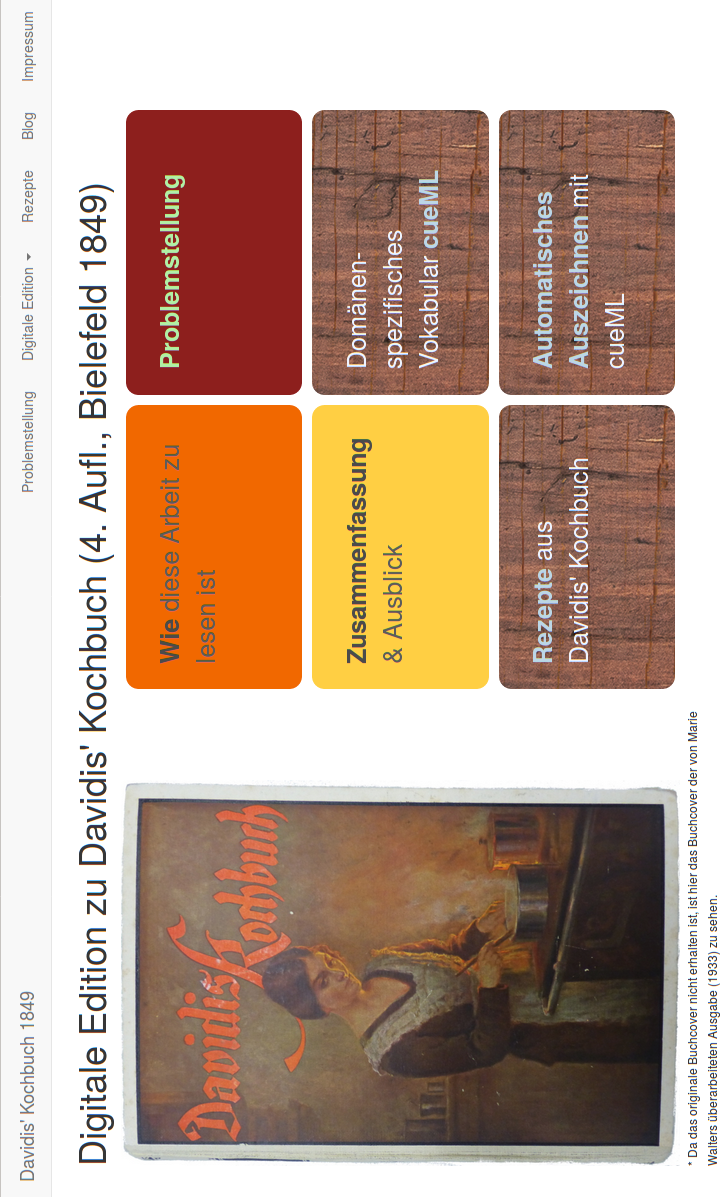
\includegraphics[width=0.98\textwidth]{WebseitenFuerDenDruck/0.png}

\includepdf[pages=-, pagecommand={}]{WebseitenFuerDenDruck/1.pdf}
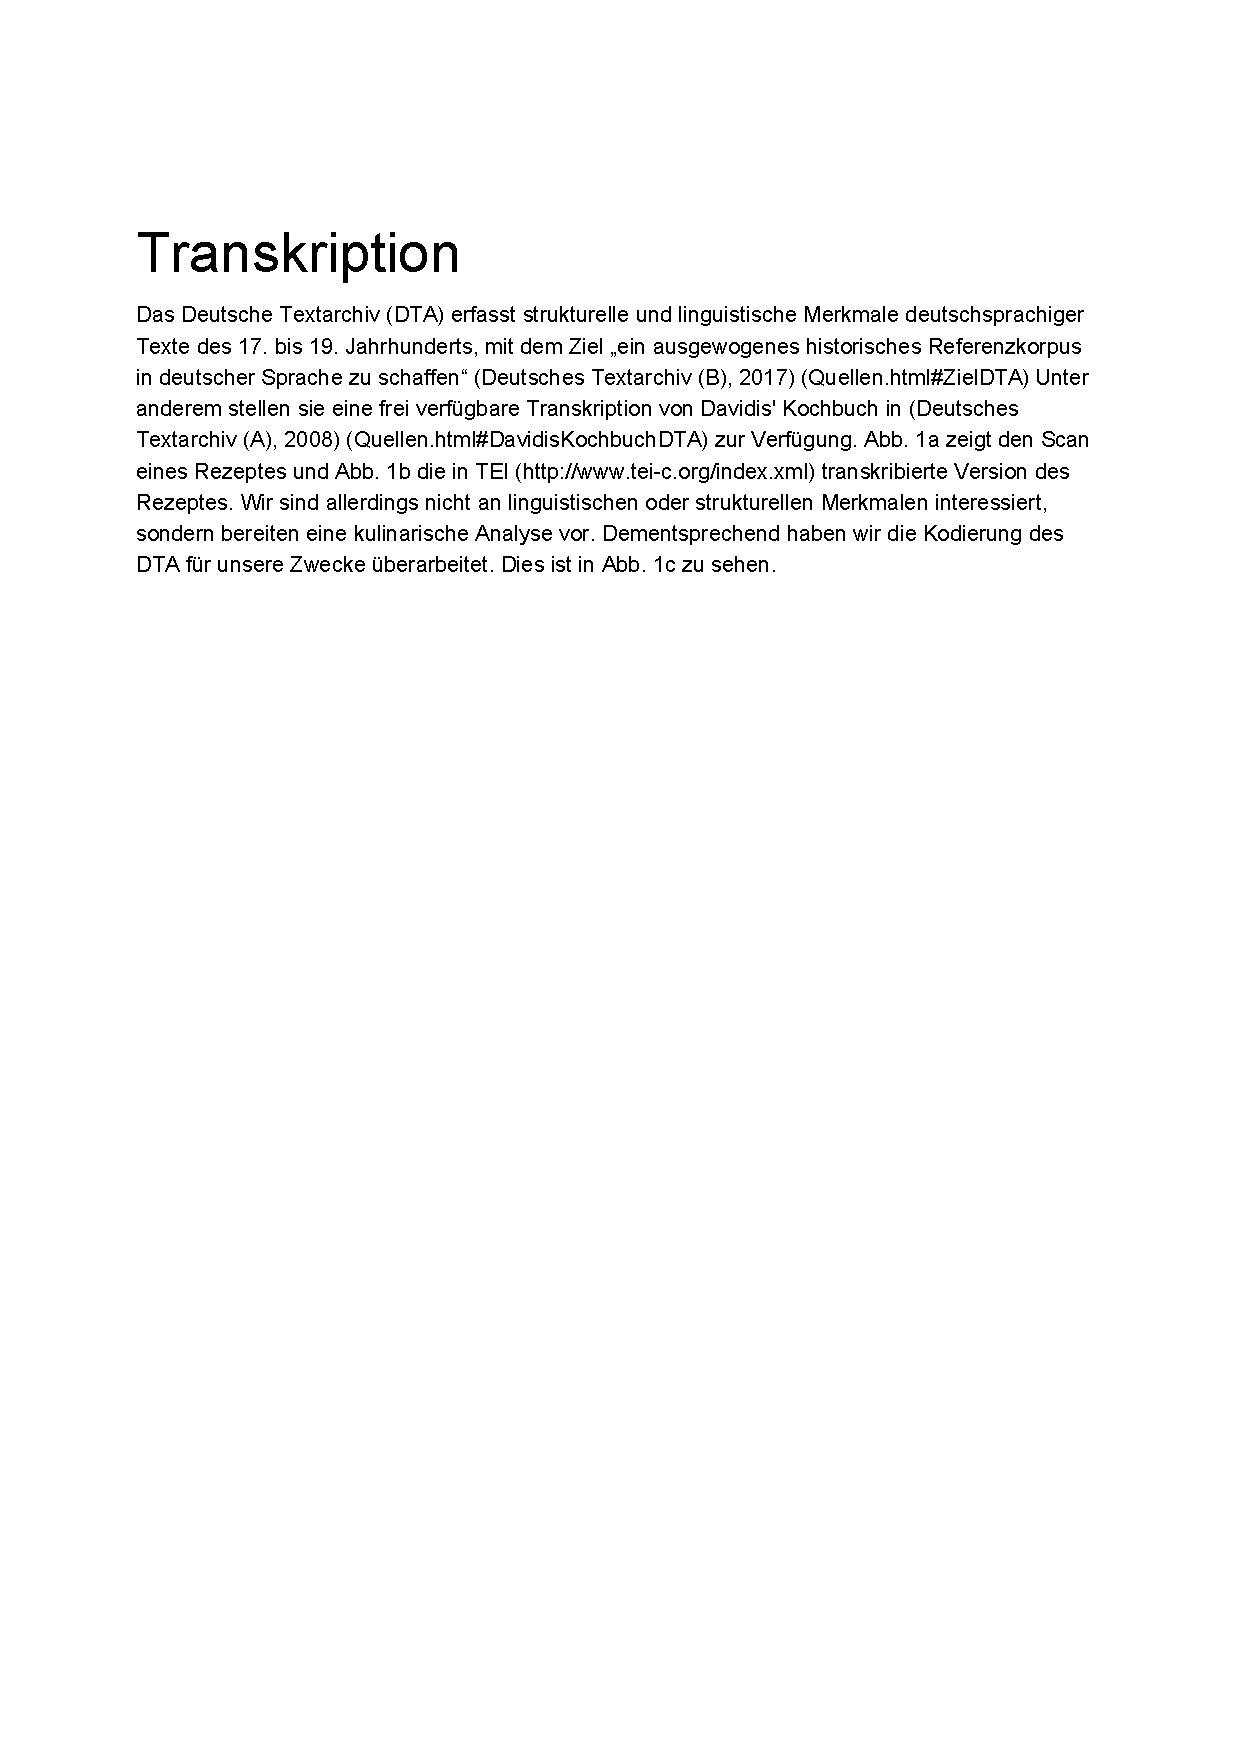
\includepdf[pages=-, pagecommand={}]{WebseitenFuerDenDruck/2.pdf}
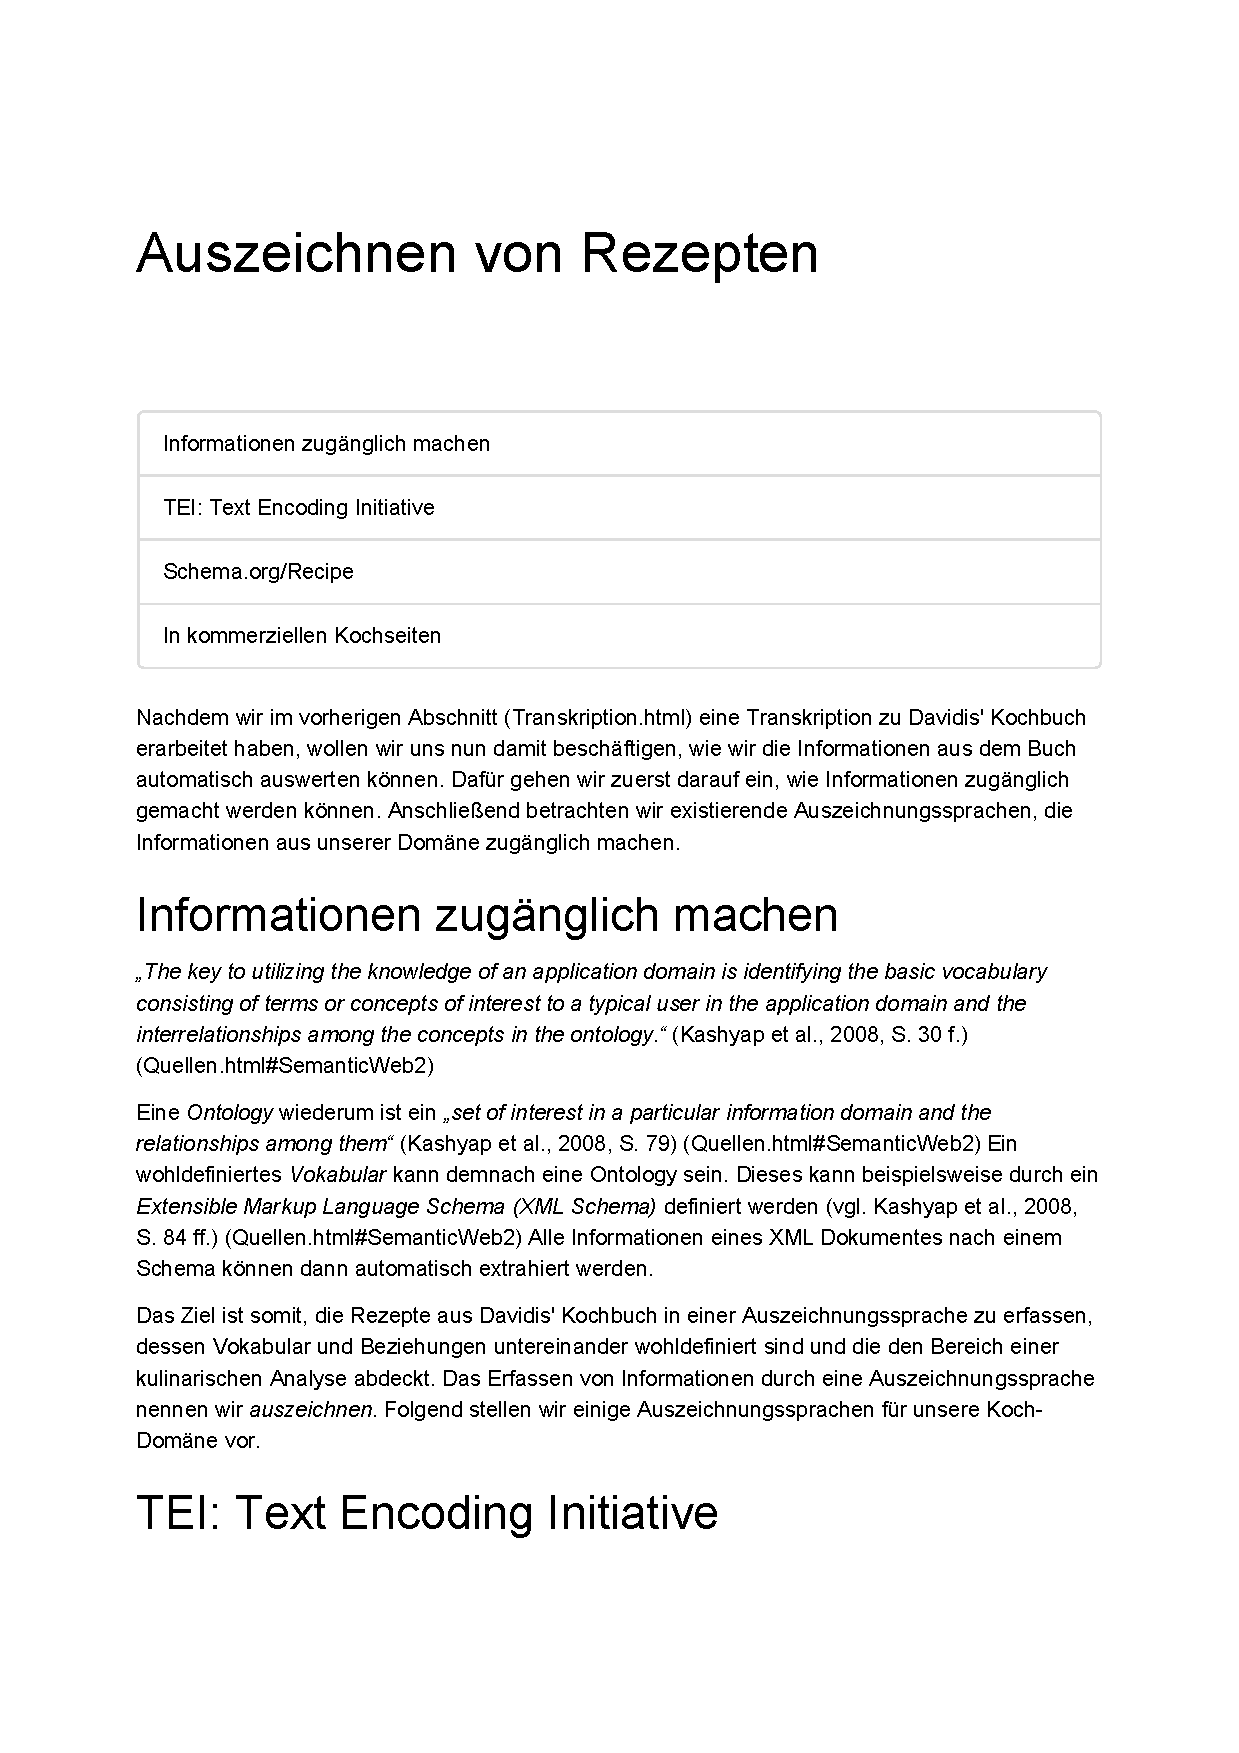
\includepdf[pages=-, pagecommand={}]{WebseitenFuerDenDruck/3.pdf}
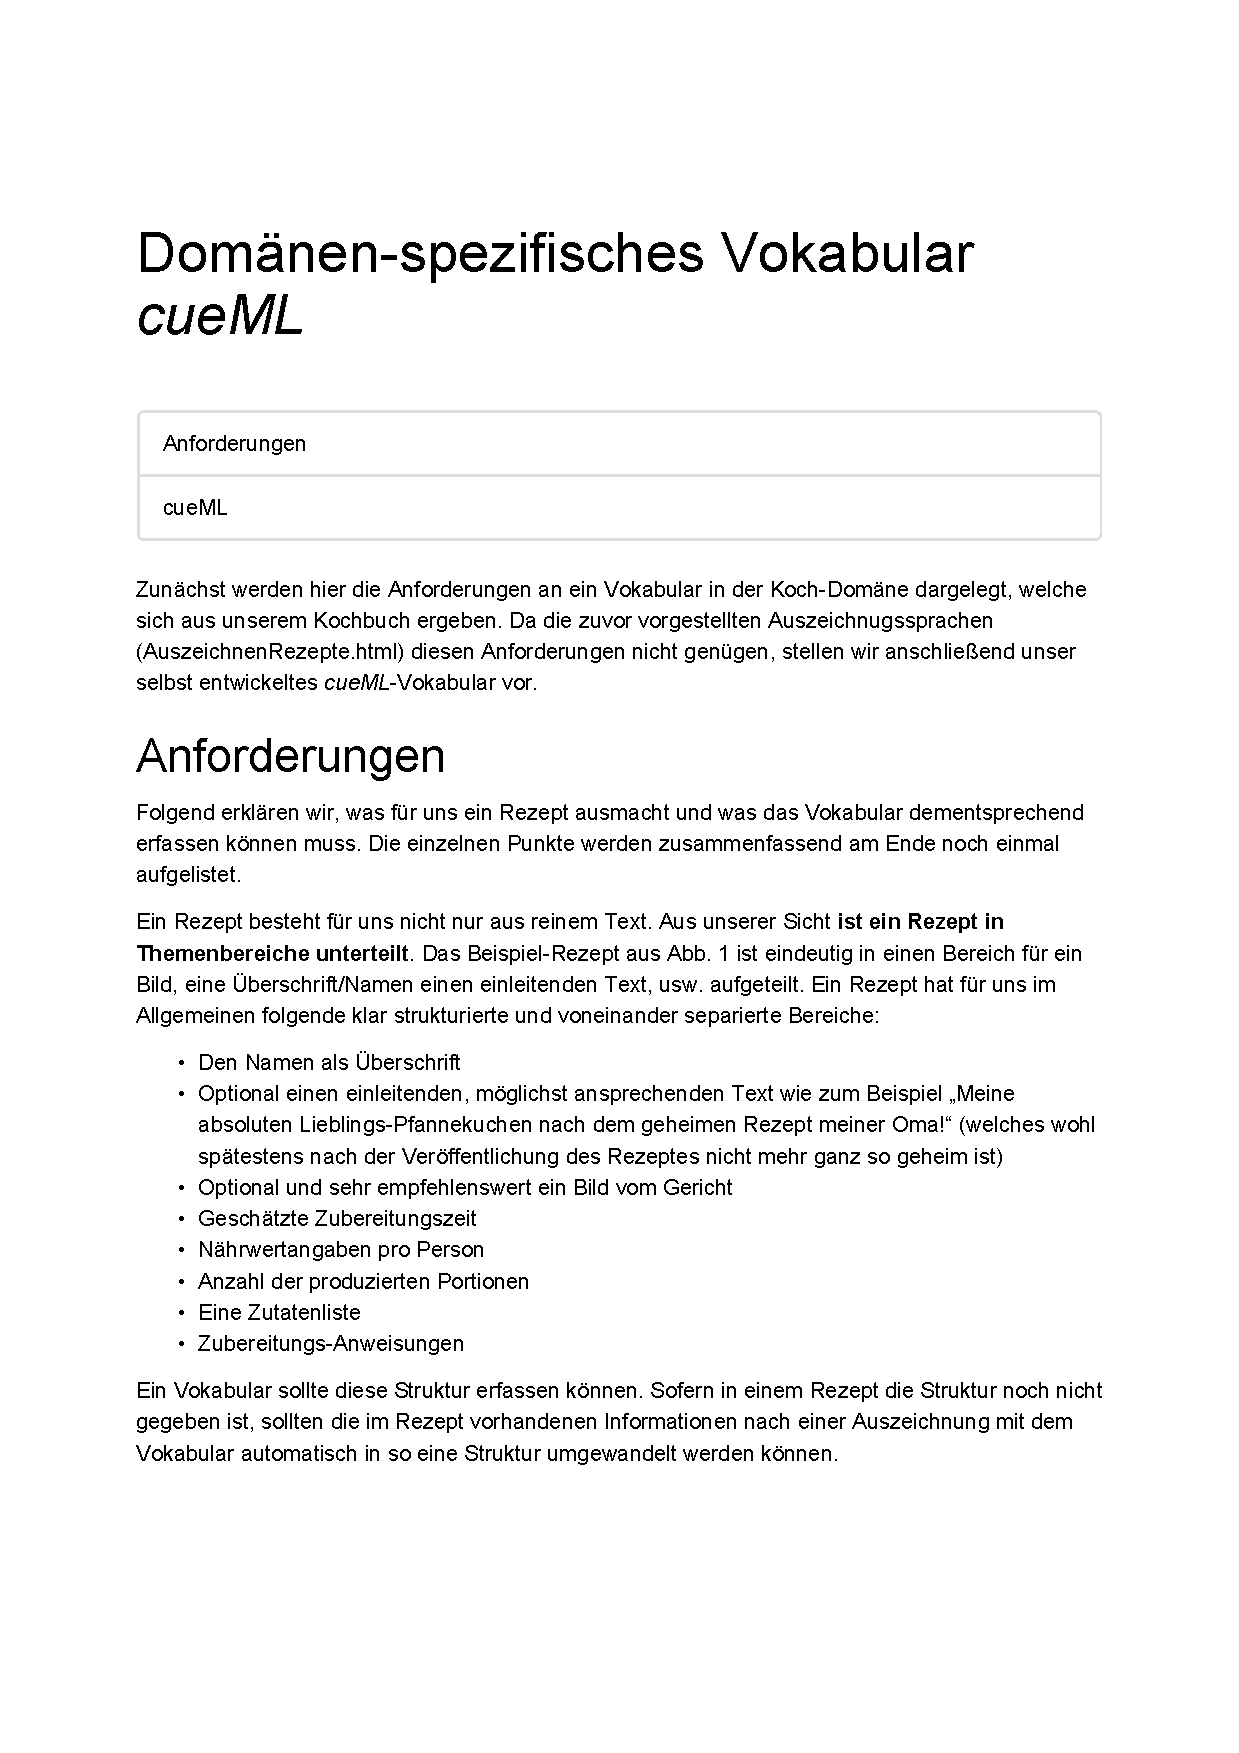
\includepdf[pages=-, pagecommand={}]{WebseitenFuerDenDruck/4.pdf}
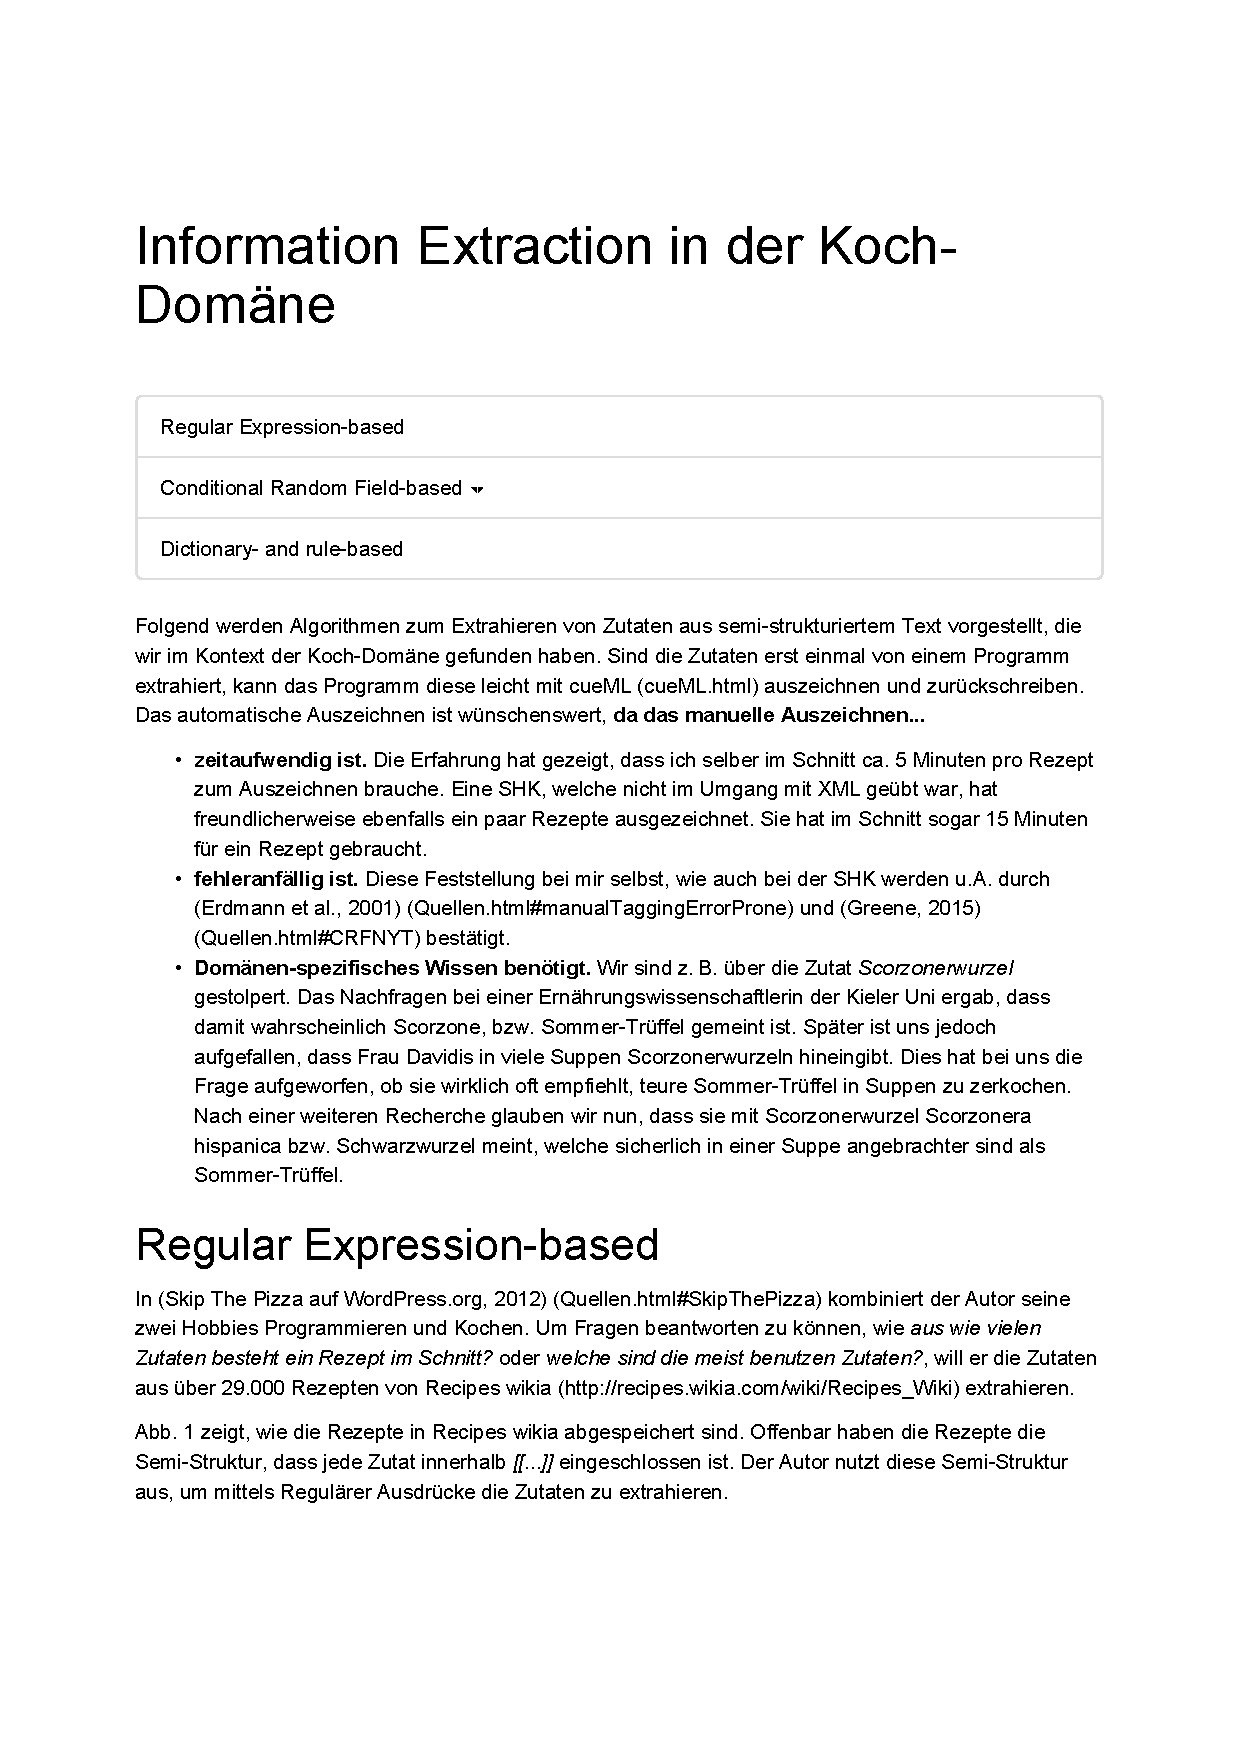
\includepdf[pages=-, pagecommand={}]{WebseitenFuerDenDruck/5.pdf}
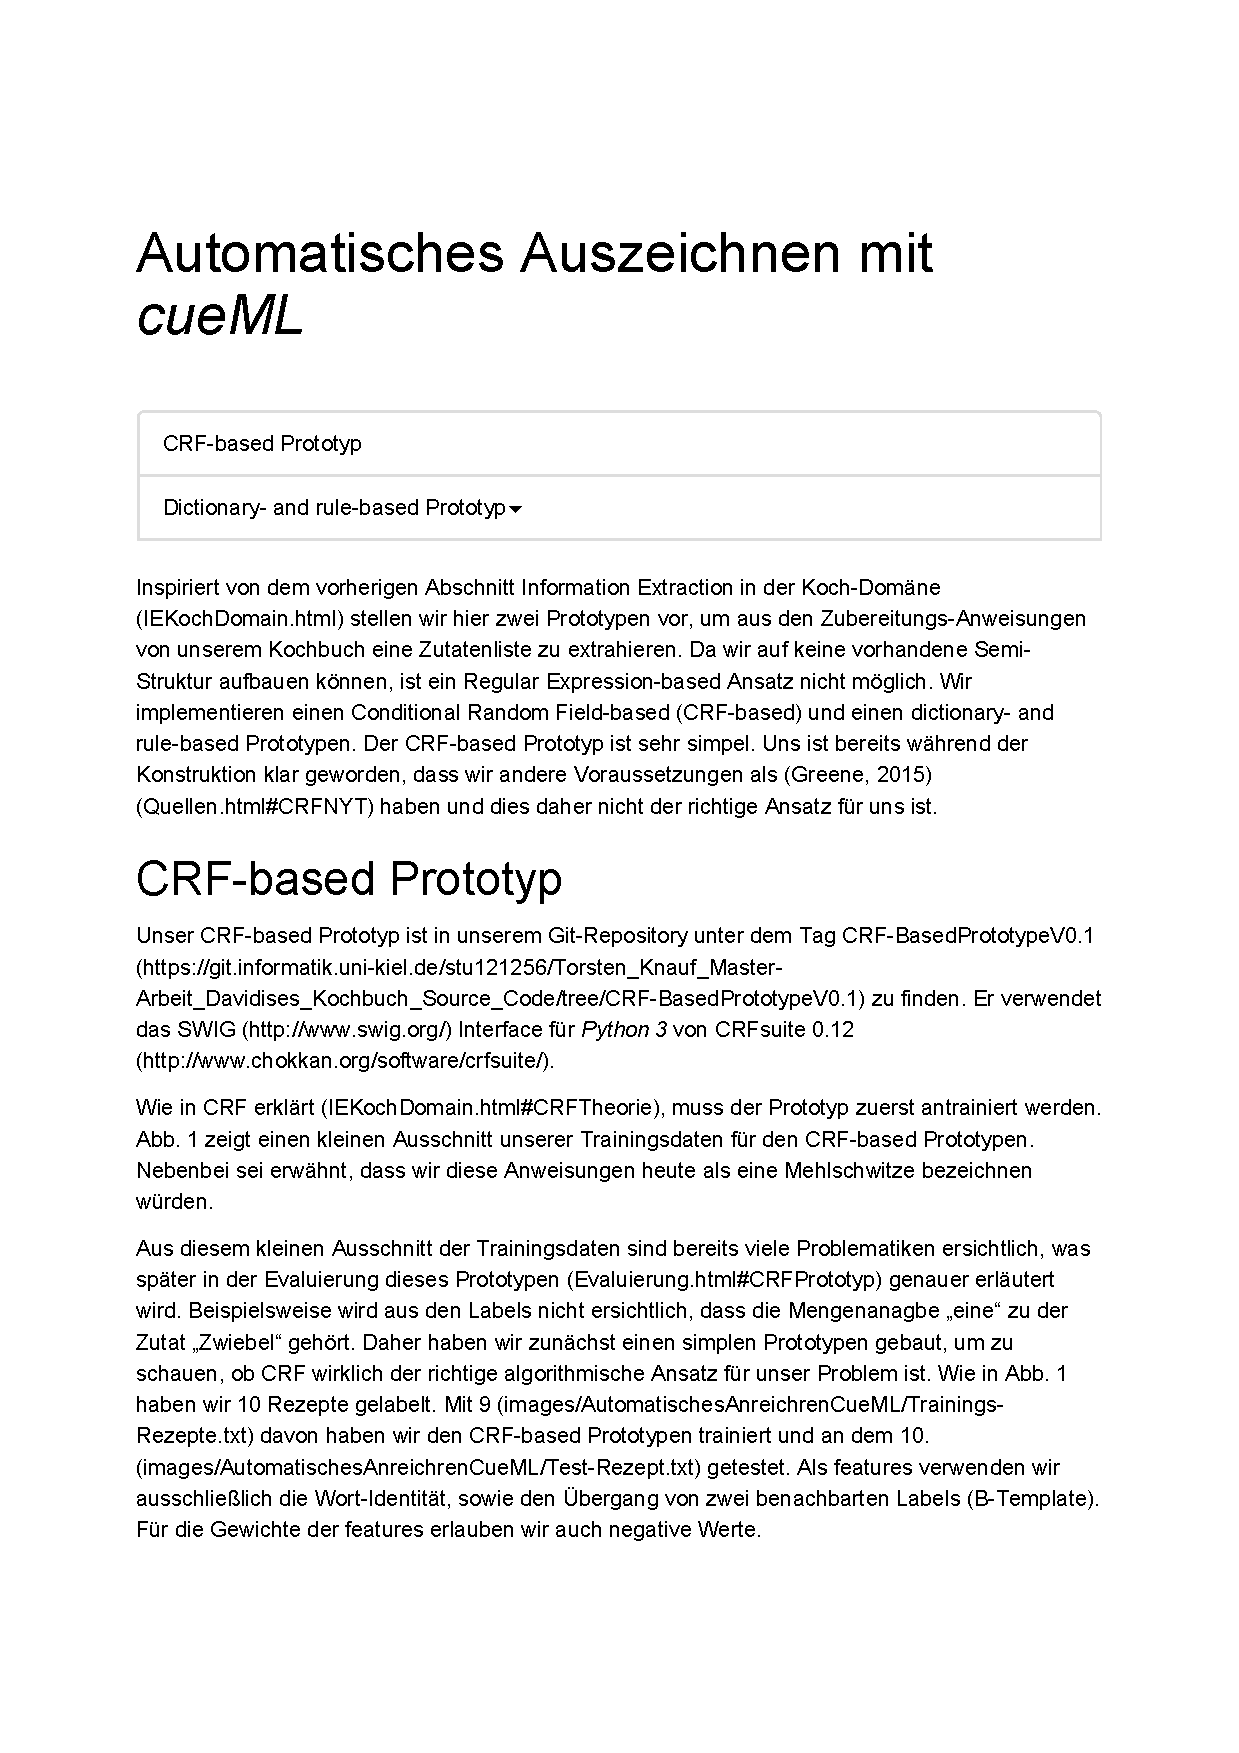
\includepdf[pages=-, pagecommand={}]{WebseitenFuerDenDruck/6.pdf}
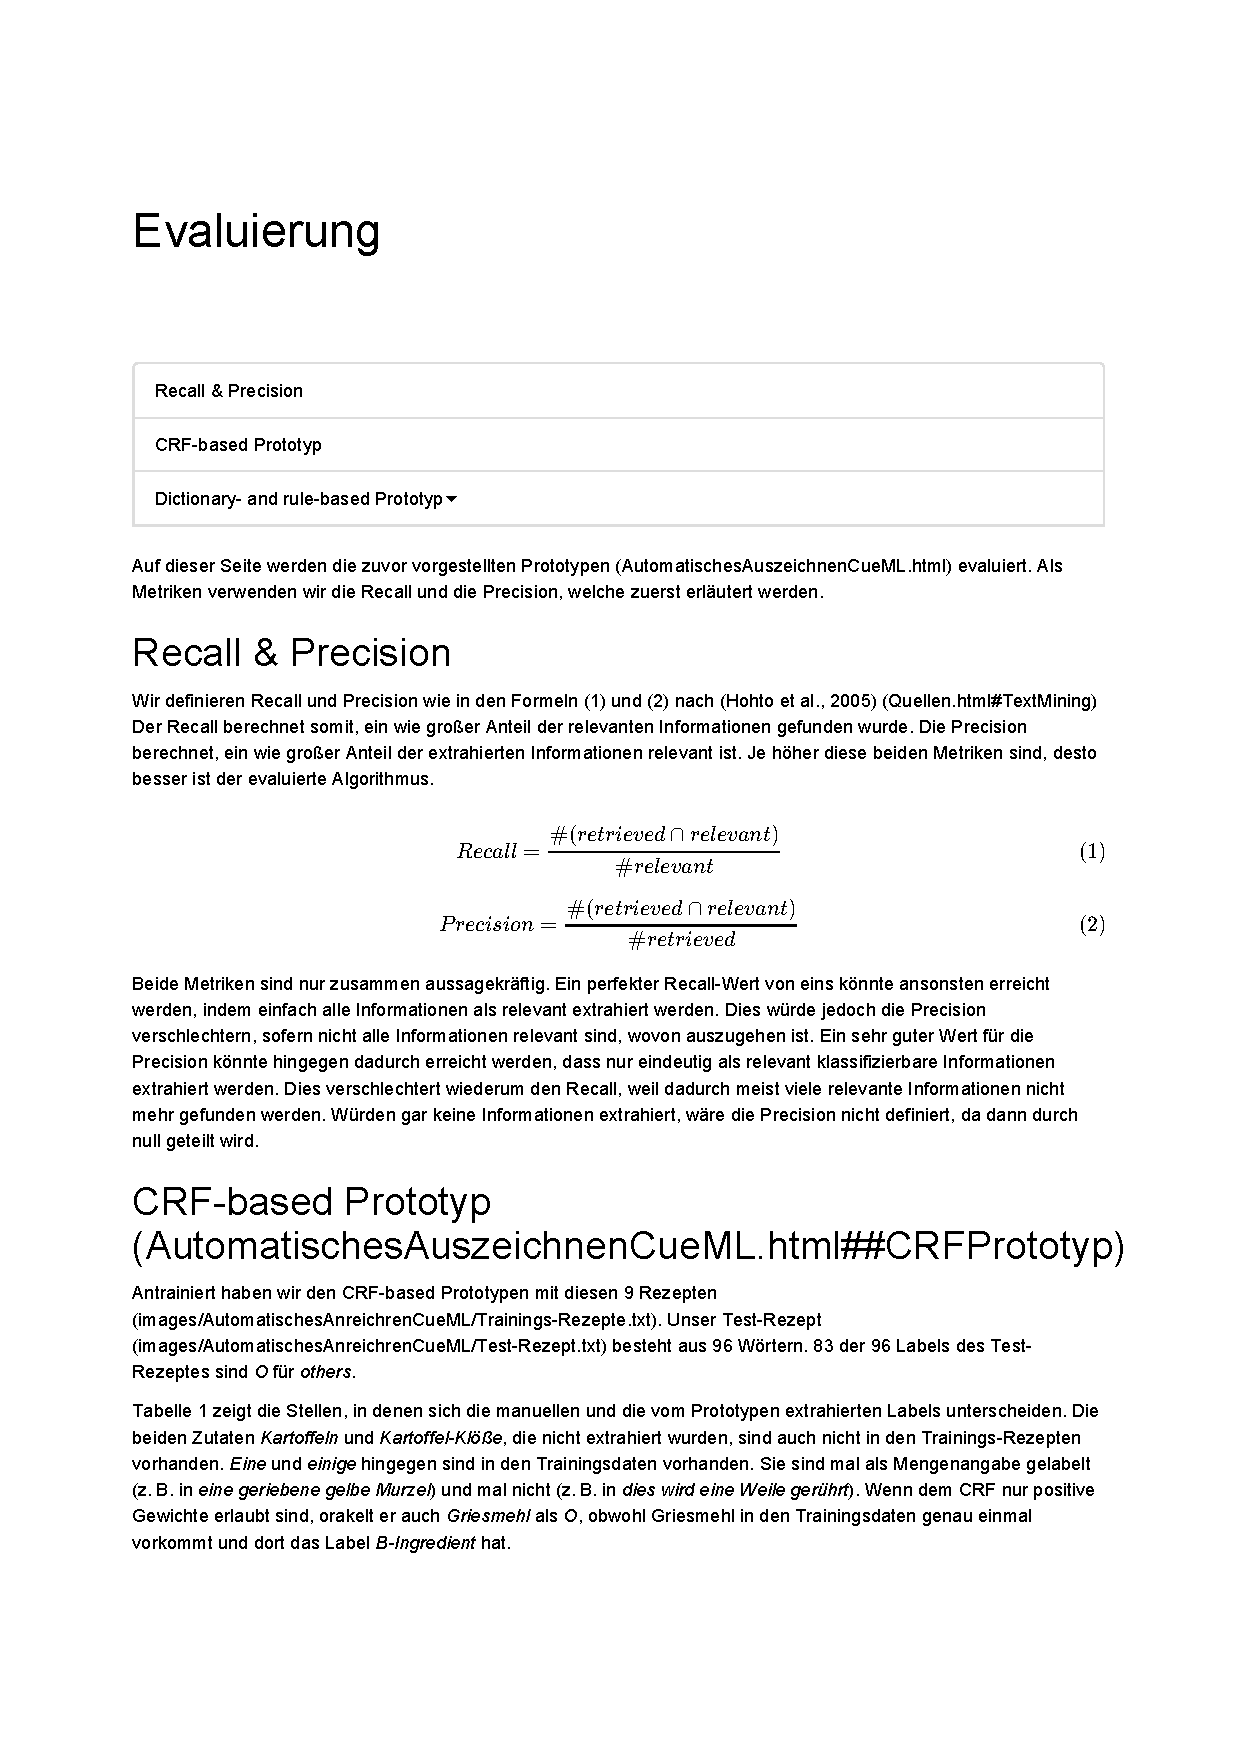
\includepdf[pages=-, pagecommand={}]{WebseitenFuerDenDruck/7.pdf}
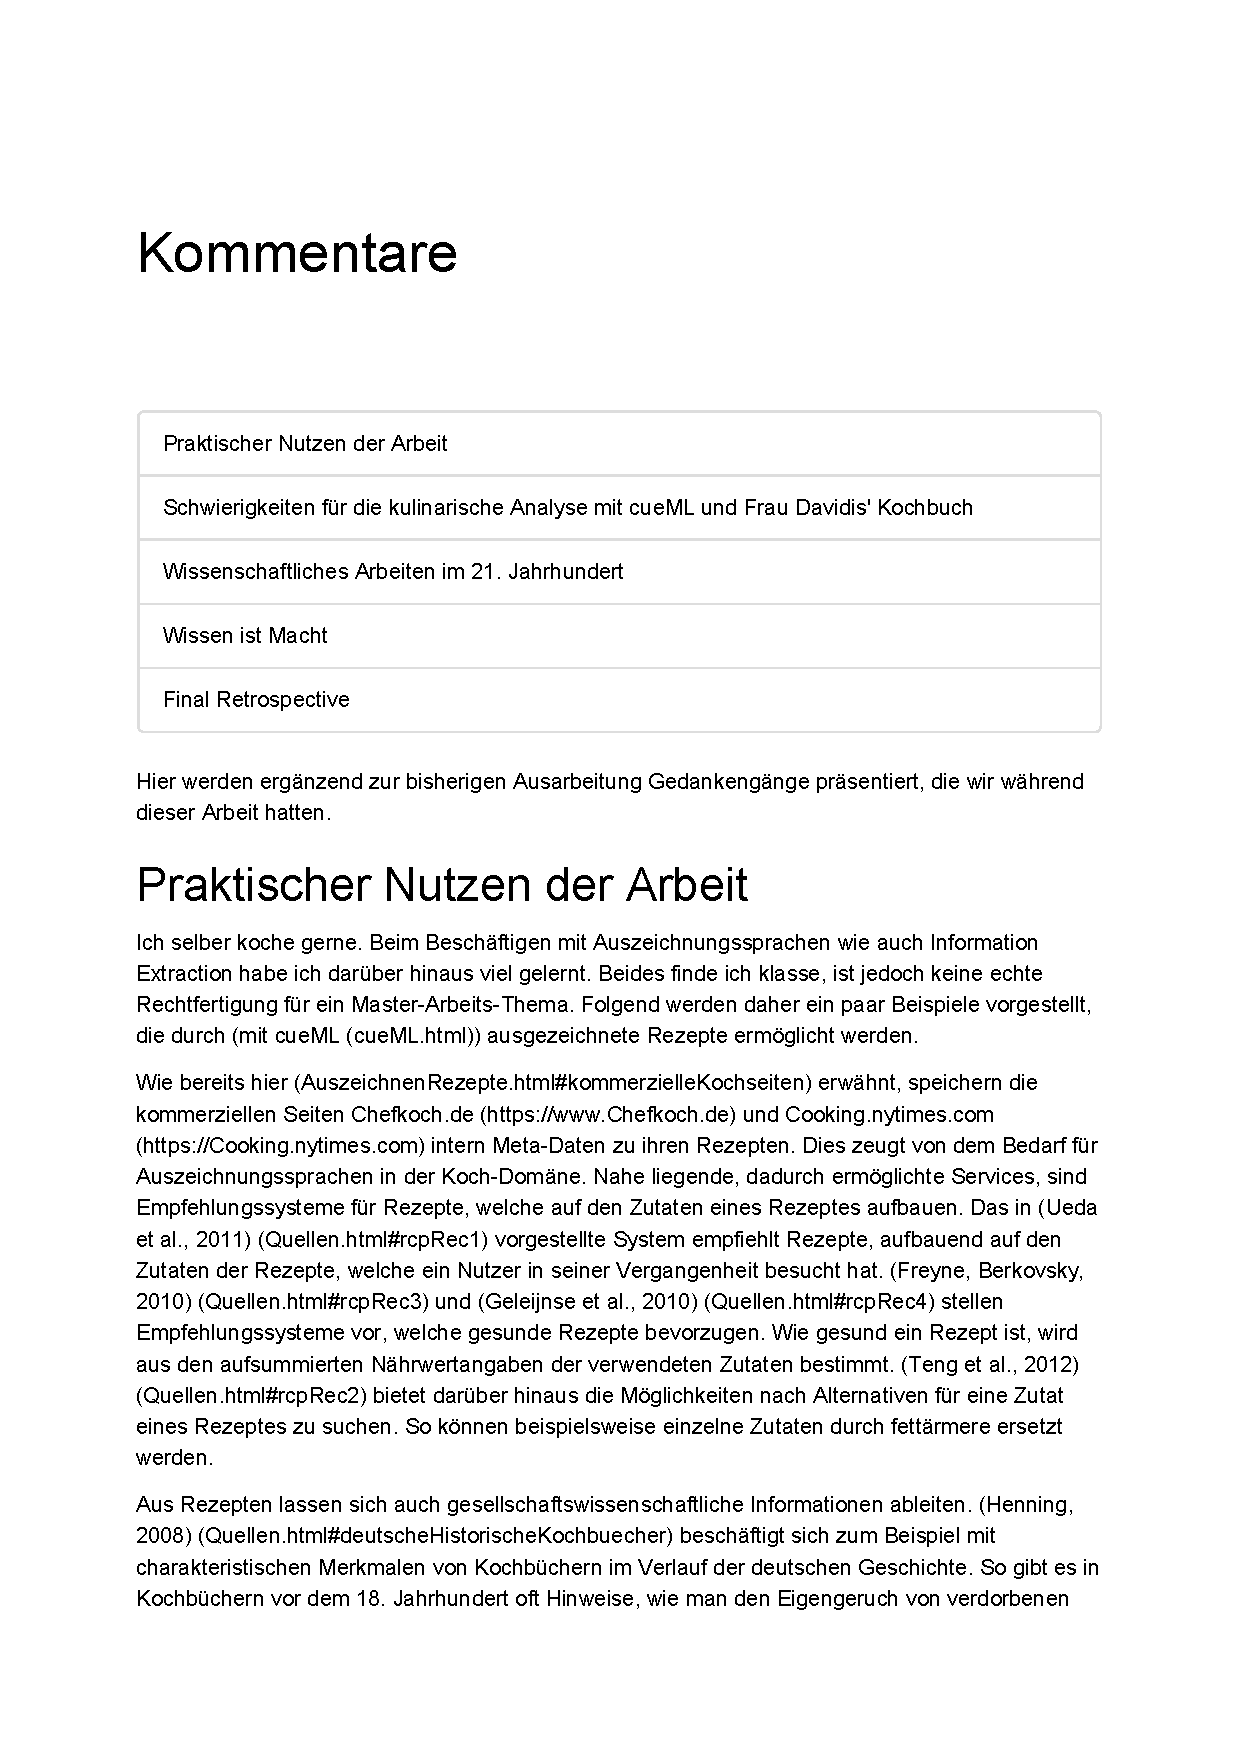
\includepdf[pages=-, pagecommand={}]{WebseitenFuerDenDruck/8.pdf}
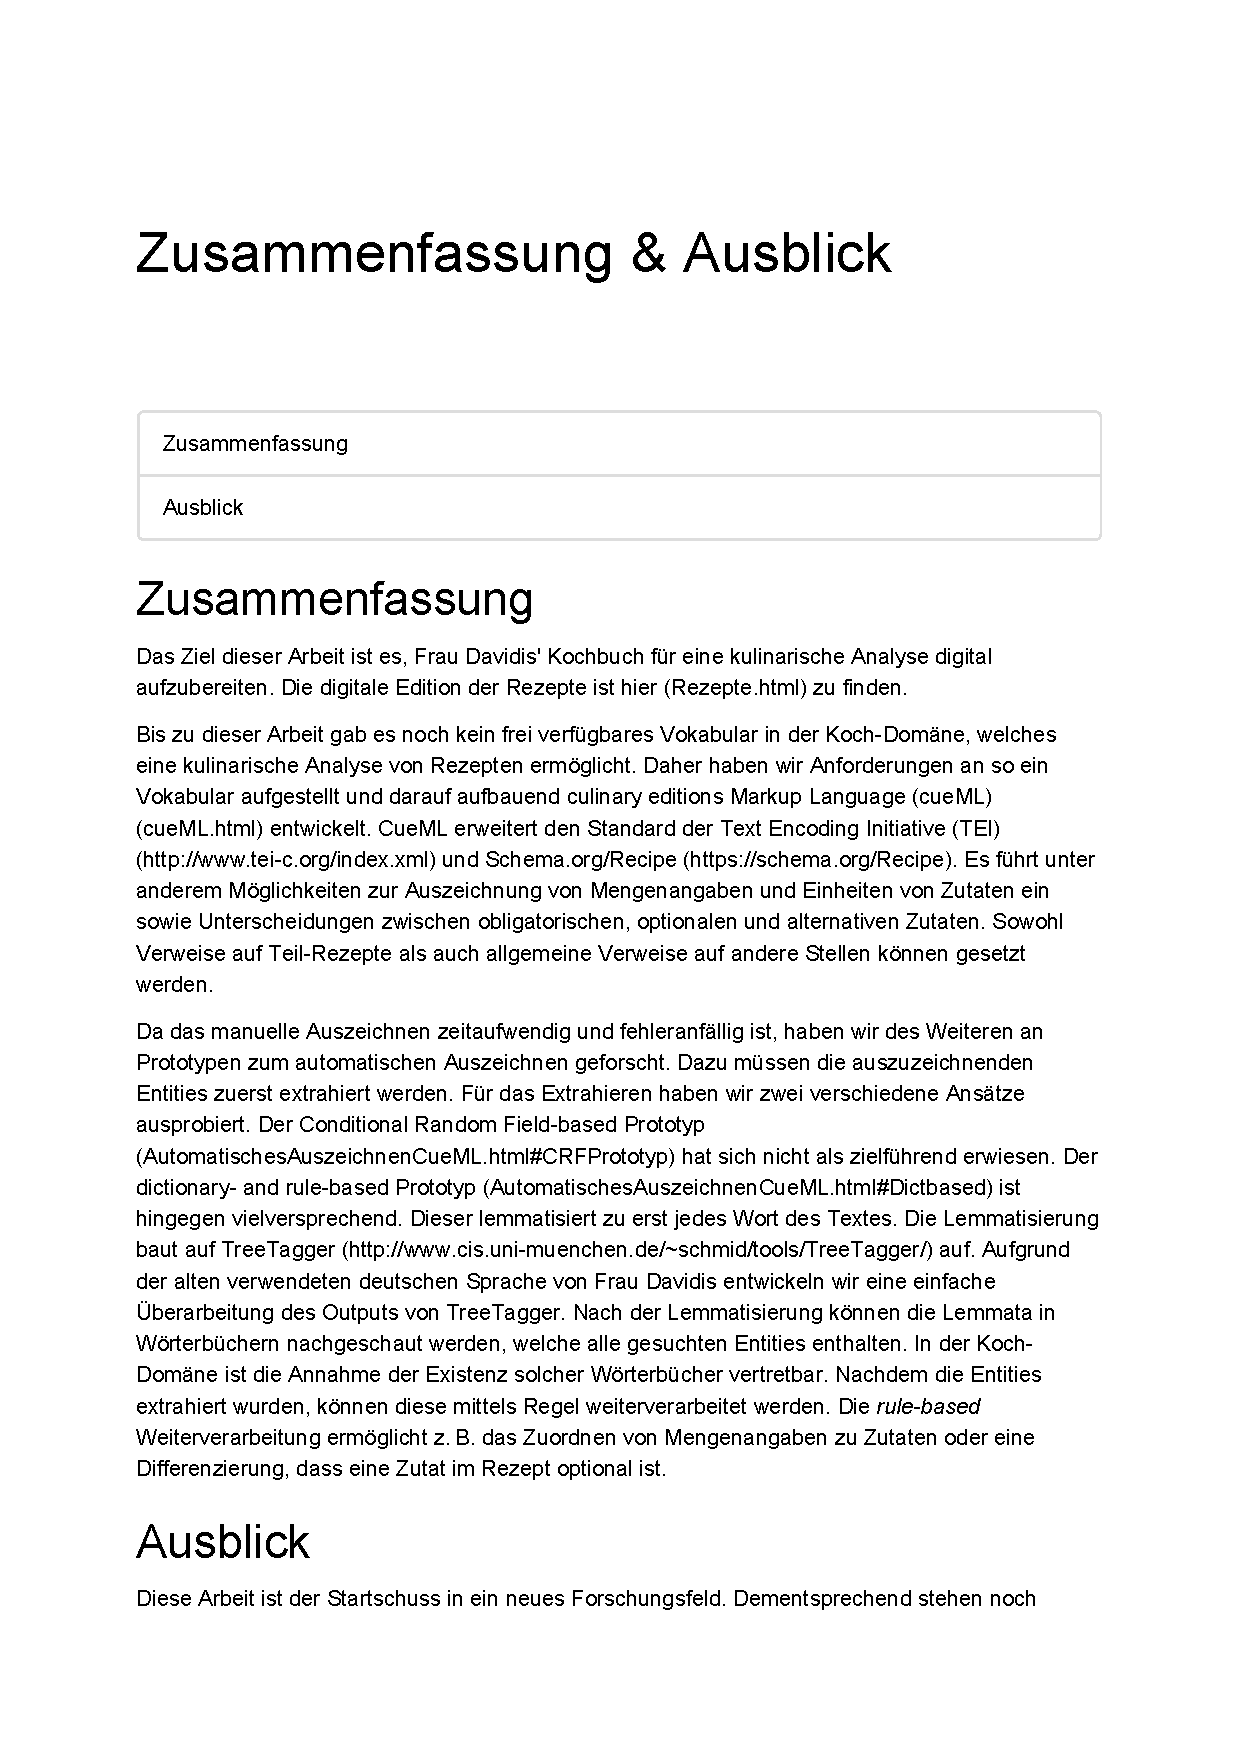
\includepdf[pages=-, pagecommand={}]{WebseitenFuerDenDruck/9.pdf}
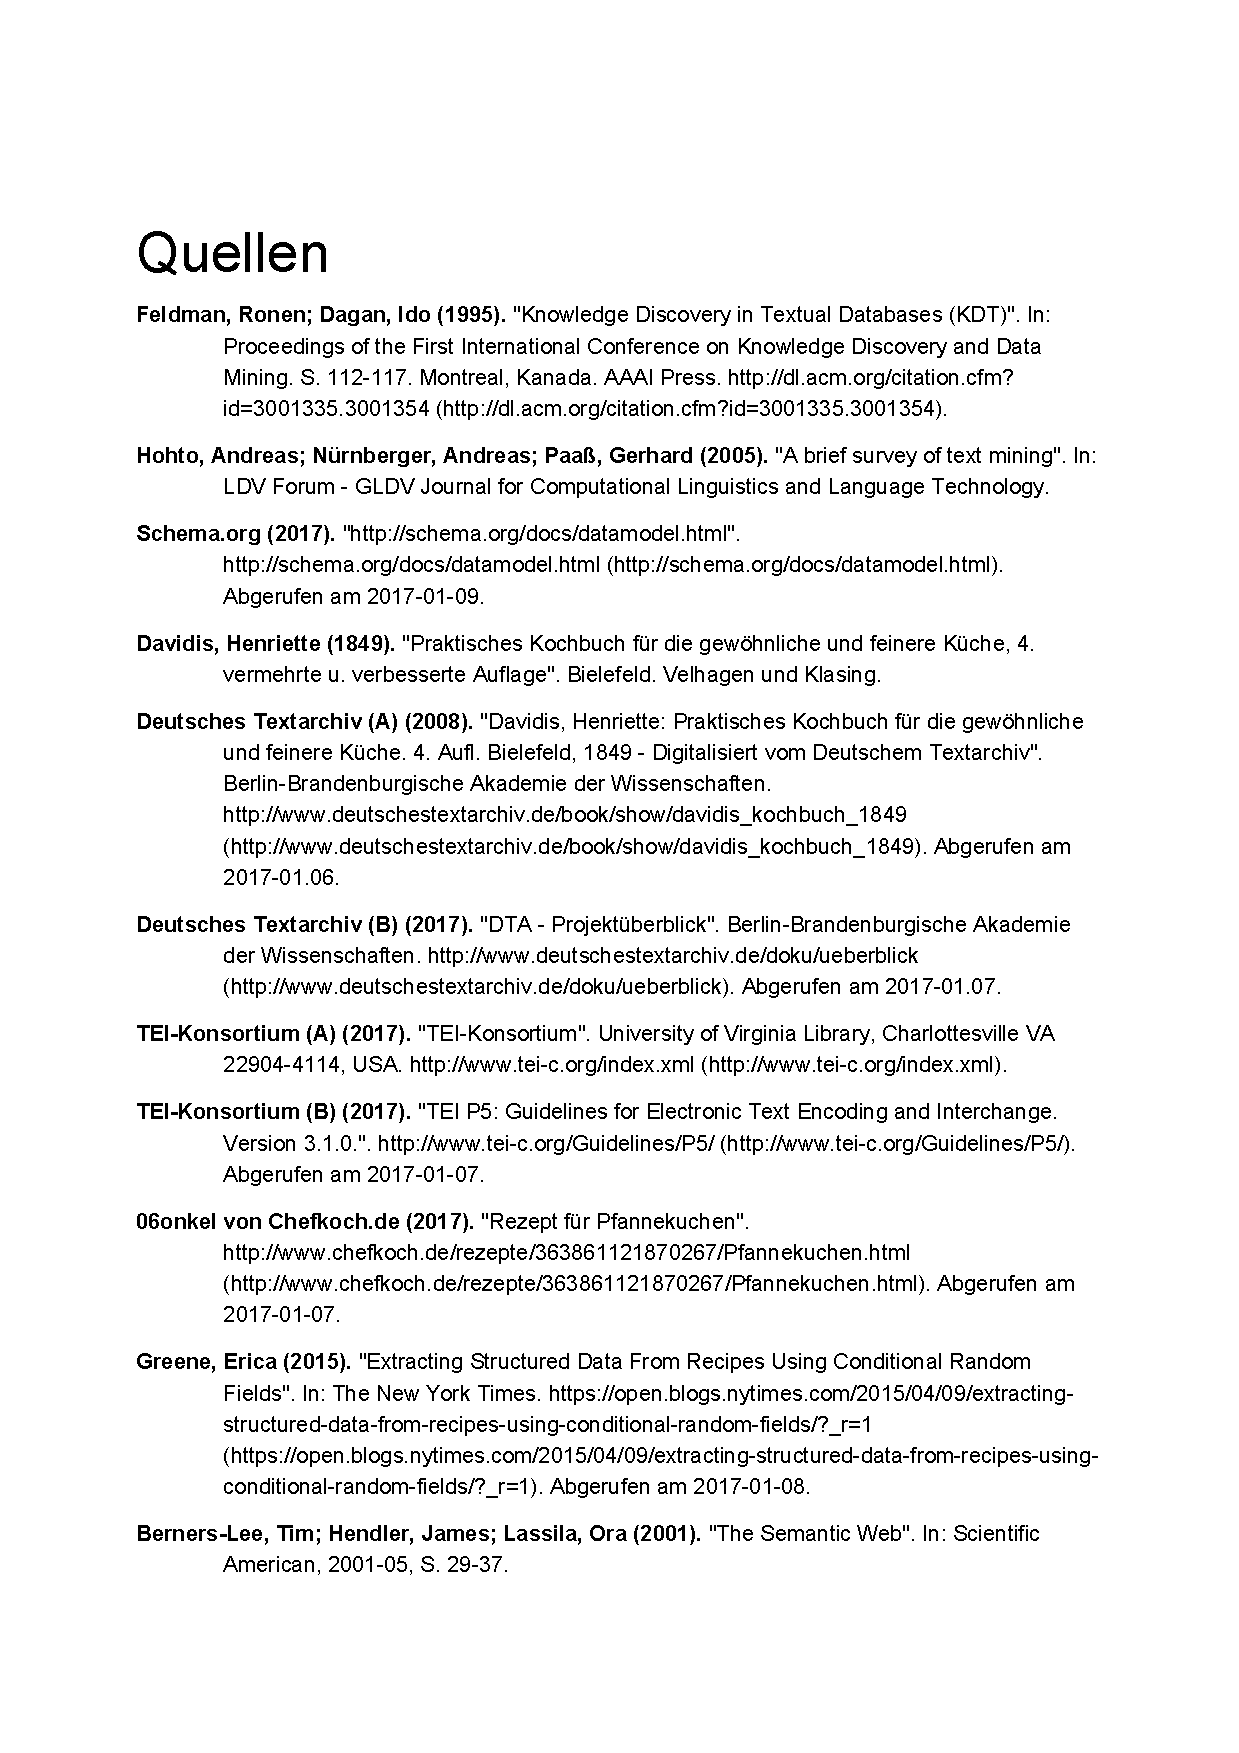
\includepdf[pages=-, pagecommand={}]{WebseitenFuerDenDruck/10.pdf}




\end{document}